\section{Durchführung}
\label{sec:Durchführung}

Der Versuchsaufbau ist in Abbildung \ref{fig:aufbau} schematisch dargestellt.
Eine Cadmium-Spektrallampe ist dem äußeren magnetischen Feld des Elektromagneten ausgesetzt.
Der restliche optische Aufbau dient zur Analyse ihres Lichtes. Der Srahl wird senkrecht zur
Magnetfeldrichtung kollimiert und trifft
auf ein Geradsichtprisma, welches das Spektrum räumlich nach den Wellenlängen auflöst.
Über den zweiten Spalt kann eine Spektrallinie ausgewählt werden und der Polarisationsfilter
filtert eine zu untersuchende Polarisation dieser Linie heraus.

\vspace{-5pt}
\begin{figure}[H]
    \centering
    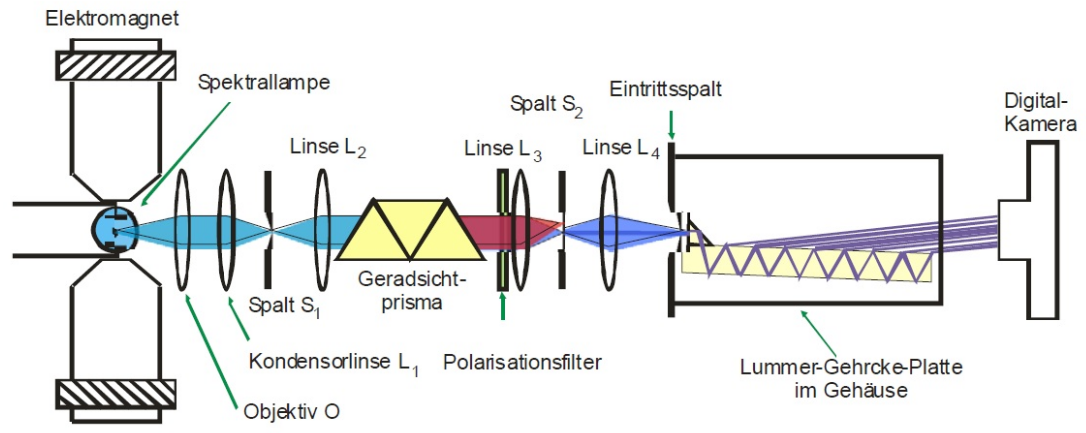
\includegraphics[scale=0.3]{content/aufbau.png}
    \caption{Versuchsaufbau der Messung \cite{alt}.}
    \label{fig:aufbau}
\end{figure}

Für Cadmium sind im wesentlichen zwei Spektrallininen zu beobachten - eine rote und eine blaue.
Anhand der roten Linie soll der normale Zeeman-Effekt und anhand der blauen der anormale 
Zeeman-Effekt untersucht werden. 

Die Wellenlängen $\lambda$ der einzelnen Spektrallinien können mithilfe der Lummer-Gehrcke-Platte 
bestimmt werden, indem ihr Interferenzverhalten verschiedener teilreflektierter Strahlen
analysiert wird. Konstruktive Interferenz tritt auf, sobald die Bragg-Bedingung

\begin{equation}
    2 \cdot d \cdot \text{cos}(\beta) = n \cdot \lambda \: , 
    \qquad n = \frac{\text{sin}(\alpha)}{\text{sin}(\beta)}
\end{equation}

mit der Plattendicke $d$ und dem Brechungsindex $n$ erfüllt ist.
Mit eingeschaltetem Magnetfeld verschieben sich die Wellenlängen der 
optischen Übergänge um $\partial \lambda$ und daraus resultierend
die Interferenzmaxima um $\partial s$.
Die maximale Differenz, die zwischen den Wellenlängen zweier Strahlen bestehen darf,
ohne dass sie sich überlagen sollen, ist definiert als Dispersionsgebiet

\vspace{-15pt}
\begin{equation}
    \Delta \lambda_\text{D} = \frac{\lambda^2}{2d} \sqrt{\frac{1}{n^2-1}}\: .
    \label{eqn:lam}
\end{equation}

Das Auflösungsvermögen der Platte lässt sich dann als

\begin{equation}
    A = \frac{\lambda}{\Delta \lambda_\text{D}} = \frac{L}{\lambda} (n^2 -1)
    \label{eqn:a}
\end{equation}

bestimmen, wobei $L$ die Plattenlänge angibt.
Zur Eichung des Elektromagneten wird die Hysterese des Magnetfeldes $\vec{B}$ in Abhängigkeit
des Feldstromes $I$ gemessen. Schließlich werden zur Bestimmung der Zeeman-Aufspaltung der
Wellenlängen die Interferenzbilder beider Spektrallinien mithilfe einer Digitalkamera
für die verschiedenen gefilterten Polarisationen aufgenommen. Damit ist auch 
eine Berechnung der Landé-Faktoren möglich.

\section{Vorbereitungsaufgaben}

\subsection{Dispersionsgebiet und Auflösungsvermögen der Lummer-Gehrcke-Platte}

Nach den Gleichungen \eqref{eqn:lam} und \eqref{eqn:a} lassen sich mithilfe
der Angaben $L = \SI{0.12}{\meter}$, $d = \SI{4}{\milli\meter}$, $n_\text{rot} = \num{1.4567}$
$n_\text{blau} = \num{1.4635}$ die Dispersionsgebiete und Auflösungsvermögen der beiden 
Spektrallinien berechnen zu

\begin{align*}
    \lambda_\text{rot} &= \SI{643.8}{\nano\meter}: & \Delta \lambda_\text{D,rot} &= \SI{48.91}{\pico\meter}\:, & A_\text{rot} &= \num{208749}\:, \\
    \lambda_\text{blau} &= \SI{480}{\nano\meter}: & \Delta \lambda_\text{D,blau} &= \SI{27.0}{\pico\meter}\:, & A_\text{blau} &= \num{285458}\:. 
\end{align*}

\subsection{Termschemata zu den Spektrallinien}

\begin{table}[H]
    %\footnotesize
    \centering
    \caption{Quantenzahlen und Landé-Faktoren der Zustände.}
    \vspace{-5pt}
    \label{tab:exp_setup}
    \begin{tabular}{c|ccc|c}
        \hline 
        Zustand & $L$ & $S$ & $J$ & $g_J$ \\
        \hline
        \hline
        $^1P_1$ & $1$ & $0$ & $1$ & $1$ \\
        $^1D_2$ & $2$ & $0$ & $2$ & $1$ \\
        $^3S_1$ & $0$ & $1$ & $1$ & $2$ \\ 
        $^3P_1$ & $1$ & $1$ & $1$ & $\sfrac{3}{2}$ \\
        \hline 
    \end{tabular}
    \vspace{-10pt}
\end{table}

\begin{table}[H]
    %\footnotesize
    \centering
    \caption{Quantenzahlen und Landé-Faktoren der Zustände.}
    \vspace{-5pt}
    \label{tab:exp_setup}
    \begin{tabular}{c|ccc}
        \hline 
        Übergang & $\Delta m = -1$ & $\Delta m = 0$ & $\Delta m = 1$ \\
        \hline
        \hline
        rot                 & $1$ & $0$ & $1$ \\
        blau, $m_1 = +1$    & $2$ & $0$ & $1$ \\
        blau, $m_1 = 0$     & $0$ & $1$ & $2$ \\ 
        blau, $m_1 = -1$    & $1$ & $1$ & $\sfrac{3}{2}$ \\
        \hline 
    \end{tabular}
    \vspace{-10pt}
\end{table}

\begin{figure}[H]
    \centering
    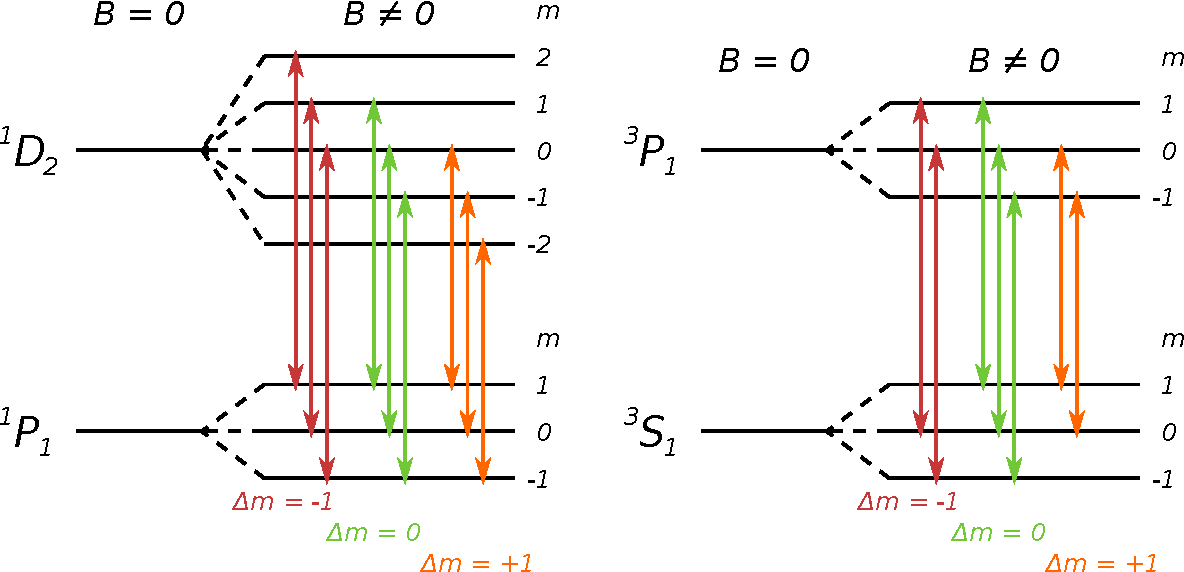
\includegraphics[scale=0.3]{content/Zeeman.pdf}
    \caption{Die Termschemata der möglichen optischen Übergänge.}
    \label{fig:term}
\end{figure}

